%%%%%%%%%%%%%%%%%%%%%%%%%%%%%%%%%%%%%%%%%
% The Legrand Orange Book
% LaTeX Template
% Version 2.4 (26/09/2018)
%
% This template was downloaded from:
% http://www.LaTeXTemplates.com
%
% Original author:
% Mathias Legrand (legrand.mathias@gmail.com) with modifications by:
% Vel (vel@latextemplates.com)
%
% License:
% CC BY-NC-SA 3.0 (http://creativecommons.org/licenses/by-nc-sa/3.0/)
%
% Compiling this template:
% This template uses biber for its bibliography and makeindex for its index.
% When you first open the template, compile it from the command line with the 
% commands below to make sure your LaTeX distribution is configured correctly:
%
% 1) pdflatex main
% 2) makeindex main.idx -s StyleInd.ist
% 3) biber main
% 4) pdflatex main x 2
%
% After this, when you wish to update the bibliography/index use the appropriate
% command above and make sure to compile with pdflatex several times 
% afterwards to propagate your changes to the document.
%
% This template also uses a number of packages which may need to be
% updated to the newest versions for the template to compile. It is strongly
% recommended you update your LaTeX distribution if you have any
% compilation errors.
%
% Important note:
% Chapter heading images should have a 2:1 width:height ratio,
% e.g. 920px width and 460px height.
%
%%%%%%%%%%%%%%%%%%%%%%%%%%%%%%%%%%%%%%%%%

%----------------------------------------------------------------------------------------
%	PACKAGES AND OTHER DOCUMENT CONFIGURATIONS
%----------------------------------------------------------------------------------------

\documentclass[11pt,fleqn]{book} % Default font size and left-justified equations

%%%%%%%%%%%%%%%%%%%%%%%%%%%%%%%%%%%%%%%%%
% The Legrand Orange Book
% Structural Definitions File
% Version 2.1 (26/09/2018)
%
% Original author:
% Mathias Legrand (legrand.mathias@gmail.com) with modifications by:
% Vel (vel@latextemplates.com)
% 
% This file was downloaded from:
% http://www.LaTeXTemplates.com
%
% License:
% CC BY-NC-SA 3.0 (http://creativecommons.org/licenses/by-nc-sa/3.0/)
%
%%%%%%%%%%%%%%%%%%%%%%%%%%%%%%%%%%%%%%%%%

%----------------------------------------------------------------------------------------
%	VARIOUS REQUIRED PACKAGES AND CONFIGURATIONS
%----------------------------------------------------------------------------------------

\usepackage{graphicx} % Required for including pictures
\graphicspath{{Pictures/}} % Specifies the directory where pictures are stored

\usepackage{lipsum} % Inserts dummy text

\usepackage{tikz} % Required for drawing custom shapes

\usepackage[english]{babel} % English language/hyphenation

\usepackage{enumitem} % Customize lists
\setlist{nolistsep} % Reduce spacing between bullet points and numbered lists

\usepackage{booktabs} % Required for nicer horizontal rules in tables

\usepackage{xcolor} % Required for specifying colors by name
\definecolor{ocre}{RGB}{243,102,25} % Define the orange color used for highlighting throughout the book

%----------------------------------------------------------------------------------------
%	MARGINS
%----------------------------------------------------------------------------------------

\usepackage{geometry} % Required for adjusting page dimensions and margins

\geometry{
	paper=a4paper, % Paper size, change to letterpaper for US letter size
	top=3cm, % Top margin
	bottom=3cm, % Bottom margin
	left=3cm, % Left margin
	right=3cm, % Right margin
	headheight=14pt, % Header height
	footskip=1.4cm, % Space from the bottom margin to the baseline of the footer
	headsep=10pt, % Space from the top margin to the baseline of the header
	%showframe, % Uncomment to show how the type block is set on the page
}

%----------------------------------------------------------------------------------------
%	FONTS
%----------------------------------------------------------------------------------------

\usepackage{avant} % Use the Avantgarde font for headings
%\usepackage{times} % Use the Times font for headings
\usepackage{mathptmx} % Use the Adobe Times Roman as the default text font together with math symbols from the Sym­bol, Chancery and Com­puter Modern fonts

\usepackage{microtype} % Slightly tweak font spacing for aesthetics
\usepackage[utf8]{inputenc} % Required for including letters with accents
\usepackage[T1]{fontenc} % Use 8-bit encoding that has 256 glyphs

%----------------------------------------------------------------------------------------
%	BIBLIOGRAPHY AND INDEX
%----------------------------------------------------------------------------------------

\usepackage[style=numeric,citestyle=numeric,sorting=nyt,sortcites=true,autopunct=true,babel=hyphen,hyperref=true,abbreviate=false,backref=true,backend=biber]{biblatex}
\addbibresource{bibliography.bib} % BibTeX bibliography file
\defbibheading{bibempty}{}

\usepackage{calc} % For simpler calculation - used for spacing the index letter headings correctly
\usepackage{makeidx} % Required to make an index
\makeindex % Tells LaTeX to create the files required for indexing

%----------------------------------------------------------------------------------------
%	MAIN TABLE OF CONTENTS
%----------------------------------------------------------------------------------------

\usepackage{titletoc} % Required for manipulating the table of contents

\contentsmargin{0cm} % Removes the default margin

% Part text styling (this is mostly taken care of in the PART HEADINGS section of this file)
\titlecontents{part}
	[0cm] % Left indentation
	{\addvspace{20pt}\bfseries} % Spacing and font options for parts
	{}
	{}
	{}

% Chapter text styling
\titlecontents{chapter}
	[1.25cm] % Left indentation
	{\addvspace{12pt}\large\sffamily\bfseries} % Spacing and font options for chapters
	{\color{ocre!60}\contentslabel[\Large\thecontentslabel]{1.25cm}\color{ocre}} % Formatting of numbered sections of this type
	{\color{ocre}} % Formatting of numberless sections of this type
	{\color{ocre!60}\normalsize\;\titlerule*[.5pc]{.}\;\thecontentspage} % Formatting of the filler to the right of the heading and the page number

% Section text styling
\titlecontents{section}
	[1.25cm] % Left indentation
	{\addvspace{3pt}\sffamily\bfseries} % Spacing and font options for sections
	{\contentslabel[\thecontentslabel]{1.25cm}} % Formatting of numbered sections of this type
	{} % Formatting of numberless sections of this type
	{\hfill\color{black}\thecontentspage} % Formatting of the filler to the right of the heading and the page number

% Subsection text styling
\titlecontents{subsection}
	[1.25cm] % Left indentation
	{\addvspace{1pt}\sffamily\small} % Spacing and font options for subsections
	{\contentslabel[\thecontentslabel]{1.25cm}} % Formatting of numbered sections of this type
	{} % Formatting of numberless sections of this type
	{\ \titlerule*[.5pc]{.}\;\thecontentspage} % Formatting of the filler to the right of the heading and the page number

% Figure text styling
\titlecontents{figure}
	[1.25cm] % Left indentation
	{\addvspace{1pt}\sffamily\small} % Spacing and font options for figures
	{\thecontentslabel\hspace*{1em}} % Formatting of numbered sections of this type
	{} % Formatting of numberless sections of this type
	{\ \titlerule*[.5pc]{.}\;\thecontentspage} % Formatting of the filler to the right of the heading and the page number

% Table text styling
\titlecontents{table}
	[1.25cm] % Left indentation
	{\addvspace{1pt}\sffamily\small} % Spacing and font options for tables
	{\thecontentslabel\hspace*{1em}} % Formatting of numbered sections of this type
	{} % Formatting of numberless sections of this type
	{\ \titlerule*[.5pc]{.}\;\thecontentspage} % Formatting of the filler to the right of the heading and the page number

%----------------------------------------------------------------------------------------
%	MINI TABLE OF CONTENTS IN PART HEADS
%----------------------------------------------------------------------------------------

% Chapter text styling
\titlecontents{lchapter}
	[0em] % Left indentation
	{\addvspace{15pt}\large\sffamily\bfseries} % Spacing and font options for chapters
	{\color{ocre}\contentslabel[\Large\thecontentslabel]{1.25cm}\color{ocre}} % Chapter number
	{}  
	{\color{ocre}\normalsize\sffamily\bfseries\;\titlerule*[.5pc]{.}\;\thecontentspage} % Page number

% Section text styling
\titlecontents{lsection}
	[0em] % Left indentation
	{\sffamily\small} % Spacing and font options for sections
	{\contentslabel[\thecontentslabel]{1.25cm}} % Section number
	{}
	{}

% Subsection text styling (note these aren't shown by default, display them by searchings this file for tocdepth and reading the commented text)
\titlecontents{lsubsection}
	[.5em] % Left indentation
	{\sffamily\footnotesize} % Spacing and font options for subsections
	{\contentslabel[\thecontentslabel]{1.25cm}}
	{}
	{}

%----------------------------------------------------------------------------------------
%	HEADERS AND FOOTERS
%----------------------------------------------------------------------------------------

\usepackage{fancyhdr} % Required for header and footer configuration

\pagestyle{fancy} % Enable the custom headers and footers

\renewcommand{\chaptermark}[1]{\markboth{\sffamily\normalsize\bfseries\chaptername\ \thechapter.\ #1}{}} % Styling for the current chapter in the header
\renewcommand{\sectionmark}[1]{\markright{\sffamily\normalsize\thesection\hspace{5pt}#1}{}} % Styling for the current section in the header

\fancyhf{} % Clear default headers and footers
\fancyhead[LE,RO]{\sffamily\normalsize\thepage} % Styling for the page number in the header
\fancyhead[LO]{\rightmark} % Print the nearest section name on the left side of odd pages
\fancyhead[RE]{\leftmark} % Print the current chapter name on the right side of even pages
%\fancyfoot[C]{\thepage} % Uncomment to include a footer

\renewcommand{\headrulewidth}{0.5pt} % Thickness of the rule under the header

\fancypagestyle{plain}{% Style for when a plain pagestyle is specified
	\fancyhead{}\renewcommand{\headrulewidth}{0pt}%
}

% Removes the header from odd empty pages at the end of chapters
\makeatletter
\renewcommand{\cleardoublepage}{
\clearpage\ifodd\c@page\else
\hbox{}
\vspace*{\fill}
\thispagestyle{empty}
\newpage
\fi}

%----------------------------------------------------------------------------------------
%	THEOREM STYLES
%----------------------------------------------------------------------------------------

\usepackage{amsmath,amsfonts,amssymb,amsthm} % For math equations, theorems, symbols, etc

\newcommand{\intoo}[2]{\mathopen{]}#1\,;#2\mathclose{[}}
\newcommand{\ud}{\mathop{\mathrm{{}d}}\mathopen{}}
\newcommand{\intff}[2]{\mathopen{[}#1\,;#2\mathclose{]}}
\renewcommand{\qedsymbol}{$\blacksquare$}
\newtheorem{notation}{Notation}[chapter]

% Boxed/framed environments
\newtheoremstyle{ocrenumbox}% Theorem style name
{0pt}% Space above
{0pt}% Space below
{\normalfont}% Body font
{}% Indent amount
{\small\bf\sffamily\color{ocre}}% Theorem head font
{\;}% Punctuation after theorem head
{0.25em}% Space after theorem head
{\small\sffamily\color{ocre}\thmname{#1}\nobreakspace\thmnumber{\@ifnotempty{#1}{}\@upn{#2}}% Theorem text (e.g. Theorem 2.1)
\thmnote{\nobreakspace\the\thm@notefont\sffamily\bfseries\color{black}---\nobreakspace#3.}} % Optional theorem note

\newtheoremstyle{blacknumex}% Theorem style name
{5pt}% Space above
{5pt}% Space below
{\normalfont}% Body font
{} % Indent amount
{\small\bf\sffamily}% Theorem head font
{\;}% Punctuation after theorem head
{0.25em}% Space after theorem head
{\small\sffamily{\tiny\ensuremath{\blacksquare}}\nobreakspace\thmname{#1}\nobreakspace\thmnumber{\@ifnotempty{#1}{}\@upn{#2}}% Theorem text (e.g. Theorem 2.1)
\thmnote{\nobreakspace\the\thm@notefont\sffamily\bfseries---\nobreakspace#3.}}% Optional theorem note

\newtheoremstyle{blacknumbox} % Theorem style name
{0pt}% Space above
{0pt}% Space below
{\normalfont}% Body font
{}% Indent amount
{\small\bf\sffamily}% Theorem head font
{\;}% Punctuation after theorem head
{0.25em}% Space after theorem head
{\small\sffamily\thmname{#1}\nobreakspace\thmnumber{\@ifnotempty{#1}{}\@upn{#2}}% Theorem text (e.g. Theorem 2.1)
\thmnote{\nobreakspace\the\thm@notefont\sffamily\bfseries---\nobreakspace#3.}}% Optional theorem note

% Non-boxed/non-framed environments
\newtheoremstyle{ocrenum}% Theorem style name
{5pt}% Space above
{5pt}% Space below
{\normalfont}% Body font
{}% Indent amount
{\small\bf\sffamily\color{ocre}}% Theorem head font
{\;}% Punctuation after theorem head
{0.25em}% Space after theorem head
{\small\sffamily\color{ocre}\thmname{#1}\nobreakspace\thmnumber{\@ifnotempty{#1}{}\@upn{#2}}% Theorem text (e.g. Theorem 2.1)
\thmnote{\nobreakspace\the\thm@notefont\sffamily\bfseries\color{black}---\nobreakspace#3.}} % Optional theorem note
\makeatother

% Defines the theorem text style for each type of theorem to one of the three styles above
\newcounter{dummy} 
\numberwithin{dummy}{section}
\theoremstyle{ocrenumbox}
\newtheorem{theoremeT}[dummy]{Theorem}
\newtheorem{problem}{Problem}[chapter]
\newtheorem{exerciseT}{Exercise}[chapter]
\theoremstyle{blacknumex}
\newtheorem{exampleT}{Example}[chapter]
\theoremstyle{blacknumbox}
\newtheorem{vocabulary}{Vocabulary}[chapter]
\newtheorem{definitionT}{Definition}[section]
\newtheorem{corollaryT}[dummy]{Corollary}
\theoremstyle{ocrenum}
\newtheorem{proposition}[dummy]{Proposition}

%----------------------------------------------------------------------------------------
%	DEFINITION OF COLORED BOXES
%----------------------------------------------------------------------------------------

\RequirePackage[framemethod=default]{mdframed} % Required for creating the theorem, definition, exercise and corollary boxes

% Theorem box
\newmdenv[skipabove=7pt,
skipbelow=7pt,
backgroundcolor=black!5,
linecolor=ocre,
innerleftmargin=5pt,
innerrightmargin=5pt,
innertopmargin=5pt,
leftmargin=0cm,
rightmargin=0cm,
innerbottommargin=5pt]{tBox}

% Exercise box	  
\newmdenv[skipabove=7pt,
skipbelow=7pt,
rightline=false,
leftline=true,
topline=false,
bottomline=false,
backgroundcolor=ocre!10,
linecolor=ocre,
innerleftmargin=5pt,
innerrightmargin=5pt,
innertopmargin=5pt,
innerbottommargin=5pt,
leftmargin=0cm,
rightmargin=0cm,
linewidth=4pt]{eBox}	

% Definition box
\newmdenv[skipabove=7pt,
skipbelow=7pt,
rightline=false,
leftline=true,
topline=false,
bottomline=false,
linecolor=ocre,
innerleftmargin=5pt,
innerrightmargin=5pt,
innertopmargin=0pt,
leftmargin=0cm,
rightmargin=0cm,
linewidth=4pt,
innerbottommargin=0pt]{dBox}	

% Corollary box
\newmdenv[skipabove=7pt,
skipbelow=7pt,
rightline=false,
leftline=true,
topline=false,
bottomline=false,
linecolor=gray,
backgroundcolor=black!5,
innerleftmargin=5pt,
innerrightmargin=5pt,
innertopmargin=5pt,
leftmargin=0cm,
rightmargin=0cm,
linewidth=4pt,
innerbottommargin=5pt]{cBox}

% Creates an environment for each type of theorem and assigns it a theorem text style from the "Theorem Styles" section above and a colored box from above
\newenvironment{theorem}{\begin{tBox}\begin{theoremeT}}{\end{theoremeT}\end{tBox}}
\newenvironment{exercise}{\begin{eBox}\begin{exerciseT}}{\hfill{\color{ocre}\tiny\ensuremath{\blacksquare}}\end{exerciseT}\end{eBox}}				  
\newenvironment{definition}{\begin{dBox}\begin{definitionT}}{\end{definitionT}\end{dBox}}	
\newenvironment{example}{\begin{exampleT}}{\hfill{\tiny\ensuremath{\blacksquare}}\end{exampleT}}		
\newenvironment{corollary}{\begin{cBox}\begin{corollaryT}}{\end{corollaryT}\end{cBox}}	

%----------------------------------------------------------------------------------------
%	REMARK ENVIRONMENT
%----------------------------------------------------------------------------------------

\newenvironment{remark}{\par\vspace{10pt}\small % Vertical white space above the remark and smaller font size
\begin{list}{}{
\leftmargin=35pt % Indentation on the left
\rightmargin=25pt}\item\ignorespaces % Indentation on the right
\makebox[-2.5pt]{\begin{tikzpicture}[overlay]
\node[draw=ocre!60,line width=1pt,circle,fill=ocre!25,font=\sffamily\bfseries,inner sep=2pt,outer sep=0pt] at (-15pt,0pt){\textcolor{ocre}{R}};\end{tikzpicture}} % Orange R in a circle
\advance\baselineskip -1pt}{\end{list}\vskip5pt} % Tighter line spacing and white space after remark

%----------------------------------------------------------------------------------------
%	SECTION NUMBERING IN THE MARGIN
%----------------------------------------------------------------------------------------

\makeatletter
\renewcommand{\@seccntformat}[1]{\llap{\textcolor{ocre}{\csname the#1\endcsname}\hspace{1em}}}                    
\renewcommand{\section}{\@startsection{section}{1}{\z@}
{-4ex \@plus -1ex \@minus -.4ex}
{1ex \@plus.2ex }
{\normalfont\large\sffamily\bfseries}}
\renewcommand{\subsection}{\@startsection {subsection}{2}{\z@}
{-3ex \@plus -0.1ex \@minus -.4ex}
{0.5ex \@plus.2ex }
{\normalfont\sffamily\bfseries}}
\renewcommand{\subsubsection}{\@startsection {subsubsection}{3}{\z@}
{-2ex \@plus -0.1ex \@minus -.2ex}
{.2ex \@plus.2ex }
{\normalfont\small\sffamily\bfseries}}                        
\renewcommand\paragraph{\@startsection{paragraph}{4}{\z@}
{-2ex \@plus-.2ex \@minus .2ex}
{.1ex}
{\normalfont\small\sffamily\bfseries}}

%----------------------------------------------------------------------------------------
%	PART HEADINGS
%----------------------------------------------------------------------------------------

% Numbered part in the table of contents
\newcommand{\@mypartnumtocformat}[2]{%
	\setlength\fboxsep{0pt}%
	\noindent\colorbox{ocre!20}{\strut\parbox[c][.7cm]{\ecart}{\color{ocre!70}\Large\sffamily\bfseries\centering#1}}\hskip\esp\colorbox{ocre!40}{\strut\parbox[c][.7cm]{\linewidth-\ecart-\esp}{\Large\sffamily\centering#2}}%
}

% Unnumbered part in the table of contents
\newcommand{\@myparttocformat}[1]{%
	\setlength\fboxsep{0pt}%
	\noindent\colorbox{ocre!40}{\strut\parbox[c][.7cm]{\linewidth}{\Large\sffamily\centering#1}}%
}

\newlength\esp
\setlength\esp{4pt}
\newlength\ecart
\setlength\ecart{1.2cm-\esp}
\newcommand{\thepartimage}{}%
\newcommand{\partimage}[1]{\renewcommand{\thepartimage}{#1}}%
\def\@part[#1]#2{%
\ifnum \c@secnumdepth >-2\relax%
\refstepcounter{part}%
\addcontentsline{toc}{part}{\texorpdfstring{\protect\@mypartnumtocformat{\thepart}{#1}}{\partname~\thepart\ ---\ #1}}
\else%
\addcontentsline{toc}{part}{\texorpdfstring{\protect\@myparttocformat{#1}}{#1}}%
\fi%
\startcontents%
\markboth{}{}%
{\thispagestyle{empty}%
\begin{tikzpicture}[remember picture,overlay]%
\node at (current page.north west){\begin{tikzpicture}[remember picture,overlay]%	
\fill[ocre!20](0cm,0cm) rectangle (\paperwidth,-\paperheight);
\node[anchor=north] at (4cm,-3.25cm){\color{ocre!40}\fontsize{220}{100}\sffamily\bfseries\thepart}; 
\node[anchor=south east] at (\paperwidth-1cm,-\paperheight+1cm){\parbox[t][][t]{8.5cm}{
\printcontents{l}{0}{\setcounter{tocdepth}{1}}% The depth to which the Part mini table of contents displays headings; 0 for chapters only, 1 for chapters and sections and 2 for chapters, sections and subsections
}};
\node[anchor=north east] at (\paperwidth-1.5cm,-3.25cm){\parbox[t][][t]{15cm}{\strut\raggedleft\color{white}\fontsize{30}{30}\sffamily\bfseries#2}};
\end{tikzpicture}};
\end{tikzpicture}}%
\@endpart}
\def\@spart#1{%
\startcontents%
\phantomsection
{\thispagestyle{empty}%
\begin{tikzpicture}[remember picture,overlay]%
\node at (current page.north west){\begin{tikzpicture}[remember picture,overlay]%	
\fill[ocre!20](0cm,0cm) rectangle (\paperwidth,-\paperheight);
\node[anchor=north east] at (\paperwidth-1.5cm,-3.25cm){\parbox[t][][t]{15cm}{\strut\raggedleft\color{white}\fontsize{30}{30}\sffamily\bfseries#1}};
\end{tikzpicture}};
\end{tikzpicture}}
\addcontentsline{toc}{part}{\texorpdfstring{%
\setlength\fboxsep{0pt}%
\noindent\protect\colorbox{ocre!40}{\strut\protect\parbox[c][.7cm]{\linewidth}{\Large\sffamily\protect\centering #1\quad\mbox{}}}}{#1}}%
\@endpart}
\def\@endpart{\vfil\newpage
\if@twoside
\if@openright
\null
\thispagestyle{empty}%
\newpage
\fi
\fi
\if@tempswa
\twocolumn
\fi}

%----------------------------------------------------------------------------------------
%	CHAPTER HEADINGS
%----------------------------------------------------------------------------------------

% A switch to conditionally include a picture, implemented by Christian Hupfer
\newif\ifusechapterimage
\usechapterimagetrue
\newcommand{\thechapterimage}{}%
\newcommand{\chapterimage}[1]{\ifusechapterimage\renewcommand{\thechapterimage}{#1}\fi}%
\newcommand{\autodot}{.}
\def\@makechapterhead#1{%
{\parindent \z@ \raggedright \normalfont
\ifnum \c@secnumdepth >\m@ne
\if@mainmatter
\begin{tikzpicture}[remember picture,overlay]
\node at (current page.north west)
{\begin{tikzpicture}[remember picture,overlay]
\node[anchor=north west,inner sep=0pt] at (0,0) {\ifusechapterimage\includegraphics[width=\paperwidth]{\thechapterimage}\fi};
\draw[anchor=west] (\Gm@lmargin,-9cm) node [line width=2pt,rounded corners=15pt,draw=ocre,fill=white,fill opacity=0.5,inner sep=15pt]{\strut\makebox[22cm]{}};
\draw[anchor=west] (\Gm@lmargin+.3cm,-9cm) node {\huge\sffamily\bfseries\color{black}\thechapter\autodot~#1\strut};
\end{tikzpicture}};
\end{tikzpicture}
\else
\begin{tikzpicture}[remember picture,overlay]
\node at (current page.north west)
{\begin{tikzpicture}[remember picture,overlay]
\node[anchor=north west,inner sep=0pt] at (0,0) {\ifusechapterimage\includegraphics[width=\paperwidth]{\thechapterimage}\fi};
\draw[anchor=west] (\Gm@lmargin,-9cm) node [line width=2pt,rounded corners=15pt,draw=ocre,fill=white,fill opacity=0.5,inner sep=15pt]{\strut\makebox[22cm]{}};
\draw[anchor=west] (\Gm@lmargin+.3cm,-9cm) node {\huge\sffamily\bfseries\color{black}#1\strut};
\end{tikzpicture}};
\end{tikzpicture}
\fi\fi\par\vspace*{270\p@}}}

%-------------------------------------------

\def\@makeschapterhead#1{%
\begin{tikzpicture}[remember picture,overlay]
\node at (current page.north west)
{\begin{tikzpicture}[remember picture,overlay]
\node[anchor=north west,inner sep=0pt] at (0,0) {\ifusechapterimage\includegraphics[width=\paperwidth]{\thechapterimage}\fi};
\draw[anchor=west] (\Gm@lmargin,-9cm) node [line width=2pt,rounded corners=15pt,draw=ocre,fill=white,fill opacity=0.5,inner sep=15pt]{\strut\makebox[22cm]{}};
\draw[anchor=west] (\Gm@lmargin+.3cm,-9cm) node {\huge\sffamily\bfseries\color{black}#1\strut};
\end{tikzpicture}};
\end{tikzpicture}
\par\vspace*{270\p@}}
\makeatother

%----------------------------------------------------------------------------------------
%	LINKS
%----------------------------------------------------------------------------------------

\usepackage{hyperref}
\hypersetup{hidelinks,backref=true,pagebackref=true,hyperindex=true,colorlinks=false,breaklinks=true,urlcolor=ocre,bookmarks=true,bookmarksopen=false}

\usepackage{bookmark}
\bookmarksetup{
open,
numbered,
addtohook={%
\ifnum\bookmarkget{level}=0 % chapter
\bookmarksetup{bold}%
\fi
\ifnum\bookmarkget{level}=-1 % part
\bookmarksetup{color=ocre,bold}%
\fi
}
}
 % Insert the commands.tex file which contains the majority of the structure behind the template

%\hypersetup{pdftitle={Title},pdfauthor={Author}} % Uncomment and fill out to include PDF metadata for the author and title of the book

%----------------------------------------------------------------------------------------
\usepackage[UTF8]{ctex}
\usepackage{graphicx}
\usepackage{float}
\usepackage{subfigure}
\usepackage{stmaryrd}
\begin{document}


%----------------------------------------------------------------------------------------
%	TITLE PAGE
%----------------------------------------------------------------------------------------

\begingroup
\thispagestyle{empty} % Suppress headers and footers on the title page
\begin{tikzpicture}[remember picture,overlay]
\node[inner sep=0pt] (background) at (current page.center) {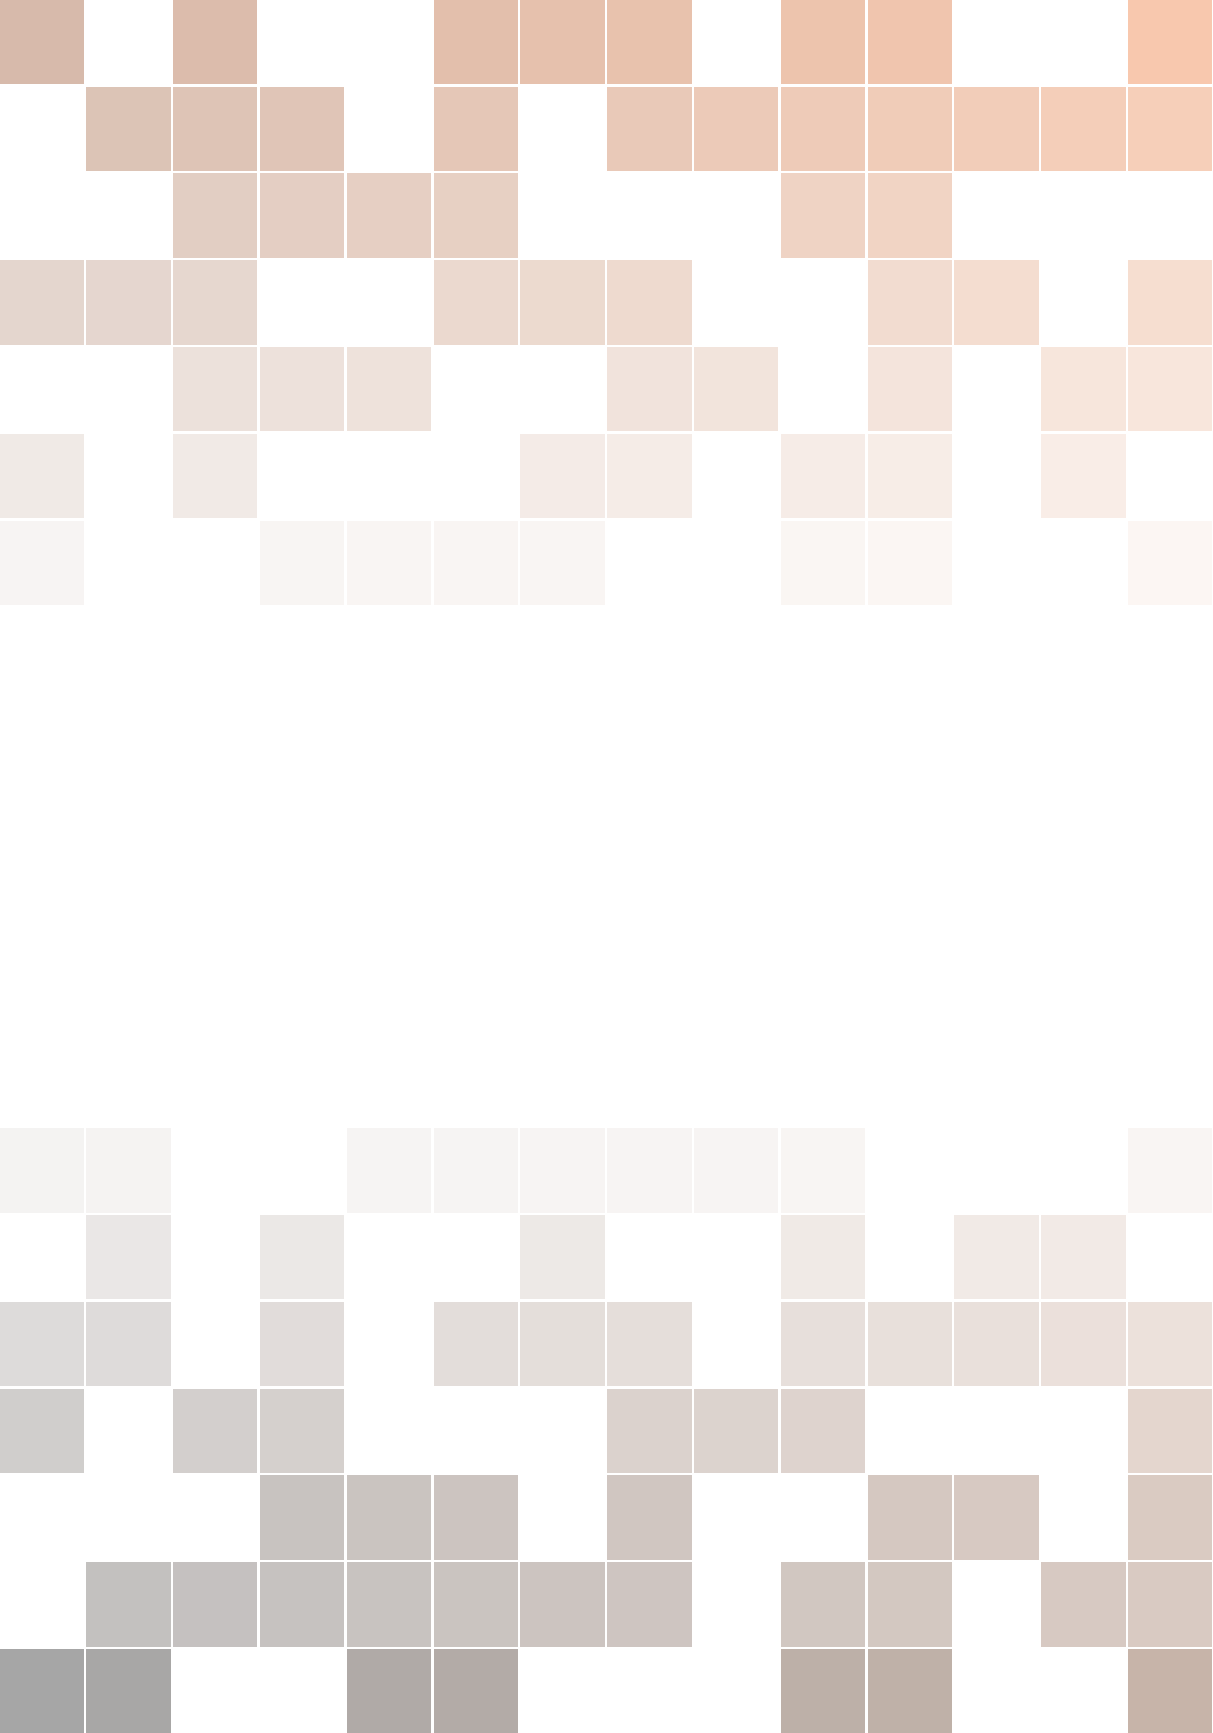
\includegraphics[width=\paperwidth]{background.pdf}};
\draw (current page.center) node [fill=ocre!30!white,fill opacity=0.6,text opacity=1,inner sep=1cm]{\Huge\centering\bfseries\sffamily\parbox[c][][t]{\paperwidth}{\centering Covid-19 tracking utilizing graph convolutional network \\[15pt] % Book title
{\Large Choujun Zhan, Jianbin Li}\\[20pt] % Subtitle
{\huge JunhuiLu, ShuntaoZhang}}}; % Author name
\end{tikzpicture}
\vfill
\endgroup

%----------------------------------------------------------------------------------------
%	COPYRIGHT PAGE
%----------------------------------------------------------------------------------------

\newpage
~\vfill
\thispagestyle{empty}

\noindent Copyright \copyright\ 2020 Li Jian Bin\\ % Copyright notice

%\noindent \textsc{Published by Publisher}\\ % Publisher

%\noindent \textsc{book-website.com}\\ % URL

\noindent Licensed under the Creative Commons Attribution-NonCommercial 3.0 Unported License (the ``License''). You may not use this file except in compliance with the License. You may obtain a copy of the License at \url{http://creativecommons.org/licenses/by-nc/3.0}. Unless required by applicable law or agreed to in writing, software distributed under the License is distributed on an \textsc{``as is'' basis, without warranties or conditions of any kind}, either express or implied. See the License for the specific language governing permissions and limitations under the License.\\ % License information, replace this with your own license (if any)

\noindent \textit{First printing, Nov 2020} % Printing/edition date

%----------------------------------------------------------------------------------------
%	TABLE OF CONTENTS
%----------------------------------------------------------------------------------------

%\usechapterimagefalse % If you don't want to include a chapter image, use this to toggle images off - it can be enabled later with \usechapterimagetrue

\chapterimage{chapter_head_1.pdf} % Table of contents heading image

\pagestyle{empty} % Disable headers and footers for the following pages

\tableofcontents % Print the table of contents itself

\cleardoublepage % Forces the first chapter to start on an odd page so it's on the right side of the book

\pagestyle{fancy} % Enable headers and footers again

%----------------------------------------------------------------------------------------
%	PART
%----------------------------------------------------------------------------------------
%----------------------------------------------------------------------------------------
%	CHAPTER 1
%----------------------------------------------------------------------------------------

\chapterimage{Cat_1.jpg} % Chapter heading image
%! Author = 207
%! Date = 2021/9/27

\part{研究背景和回顾}
    \chapter{研究背景}
        \section{研究起源}
        \section{问题描述}
        \section{研究意义}
    \chapter{现有的相关研究}
        \section{Literature Review(浓缩总结后)}
            \subsection{接触网络模型}
            \subsection{基于接触网络的传播模型}
            \subsection{防疫策略以及相关的评估标准}
        \section{阅读笔记(详细)}
            \subsection{传统的传播模型的文章阅读笔记}
            \subsection{基于Agent-based传播模型}
            \subsection{COVID-19病毒防控策略}
                COVID-19 病毒传播迅速,传染力极强,全球只有少量的国家能放置该病毒的传播,面对病毒的快速传播,不同的国家采取了不
                一样的检测措施,针对检测不同的检测对象可以分为三种方法\cite{crozier2021put}.
                \begin{itemize}
                    \item Symptomatic testing : Symptomatic testing检测策略仅对有症状的感染者进行检测,迅速对感染者追踪隔离,因此
                在检测率上往往有较高的准确率。目前使用该策略的国家有日本。
                    \item asymptomatic testing : asymptomatic testing 是一种针对无症状感染者的检测策略,这类方法目前是多数国家普遍采取的检测措施,并且不同的国家会针对不同的人群进行检测,英国和奥地利专注于定期检测保护易感染人群,
                    高风险地区。德国和比利时专注于对无症状感染者在5-7天进行每日检测,这类检测策略可以维持了成本和防疫力度的初步方法,对高
                    风险地区进行检测可以大大提高检测命中率,但是,随着时间的推移以及感染人数的增加,该方法的可行性还有待证明。
                    \item Mass testing: Mass testing大量的对社区的所有人群检测,或者对少量人口停止社区活动并进行重复性的检测。
                目前使用这类方法的有中国和越南,这类方法可以高效的控制病毒的传播,从而有效的抵御疫情,然而,这种方法成本极高,
                对于一些经济实力较弱的国家很难长期执行,一旦出现短时间内超级传播者经过多个地区进行全市甚至全省的检测,便需要极高的成本。
                \end{itemize}
                以上的三种方法在实际生活呈现出不同的状况。除了中国坚持Mass testing的方法使得整个国家仅有少数的个体感染外,其他的
                方法并没有。尽管Mass testing是真正意义上控制了感染人数的增长,然而这需要大量的劳动力成本和材料成本。
                因此,提高检测效率和降低成本扮演着控制病毒传播的关键地位,目前大量的研究针对经济和疫情的控制之间的平衡做出了相关的研究。

                [\cite{kolumbus2021effectiveness}] 提出了一个在多种高效干预措施下的SEIR的仿真模型,目的是权衡经济影响和健康之间的
                联系。在模型的模拟方面,作者模仿了现实情况,设置了一个E-R网络,每个节点的平均度为3.6(在没有任何干预
                下他引用别人的文章说是合理的),病人的平均潜伏期和平均感染期分别设置了6,8天,而感染率q = 0.5,
                病发概率为$p_{symp} = 1 - q^{1/8}$,总节点数10000,整个实验模型模拟了540天。在干预措施上
                作者在Lockdowns下按概率切断节点之间的边,也就是说,封锁程度0.3意味着存在连边的两个节点的边可能
                有30\%的概率会切断,针对隔离和追踪措施的干预下,对感染者的直接接触者进行检测,只隔离检测呈阳性的人。
                此外,作者使用封锁程度来衡量劳动力的损失情况,即考虑到的只是封锁程度与劳动力存在线性关系。
                结果表明,检测和隔离的结合能有效的减少经济经济成本呢死亡率,但是大量的检测有显著的效果。
                跟踪结合适度的测试能力可以在没有封锁的情况下实现遏制。(copy)
                跟踪和检测结合起来以降低死亡率和经济成本的政策极其有用,它们有可能在不施加任何社交距离限制的情况下遏制疫情。
                这突出了交易的棘手的社会问题——这些收益与病人的隐私相冲突,追踪不可避免地侵犯了病人的隐私。

                [\cite{eilersen2020cost}] 专注于衡量在有限的隔离与检测的情况下减缓成本收益 同样地使用SEIR仿真模型进行研究,但作者不仅将个体分为30\%Work,40\%Family,15\%Friends,15\%Public,
                而且在状态的持续时间有所调整,令S,I,R的状态平均维持在时间3天,从E到I的平均时间为5天,其中有一半的时间
                维持着E的状态,后半段时间维持Pre-symptomatic(infectious)的过度状态。在个体的设置上是模仿了丹麦的人口
                分布,平均每个个体有2位亲人,10位工友,两组朋友每组有5位。每个个体每一轮(0.5day)拥有一定概率抽到扮演着这4中
                角色的机会,总共5000个个体,最后感染率的设置是美国死亡率 + 23\%。结果表明,图\ref{fig:paper_result1}是实验的结果,
                减少工作、社交接触、减少工作间的规模程度能有效的延缓并降低感染人数。接着,作者使用 1 step tracing
                and quarantine strategy(1STQ)策略,即
                \begin{itemize}
                    \item close the workplaces of people who are tested positive for the disease.
                    \item isolate their regular social contacts for a limited period
                    \item keep symptomatic individuals in quarantine until they recover.
                \end{itemize}
                \begin{figure}[htbp]
                    \centering
                    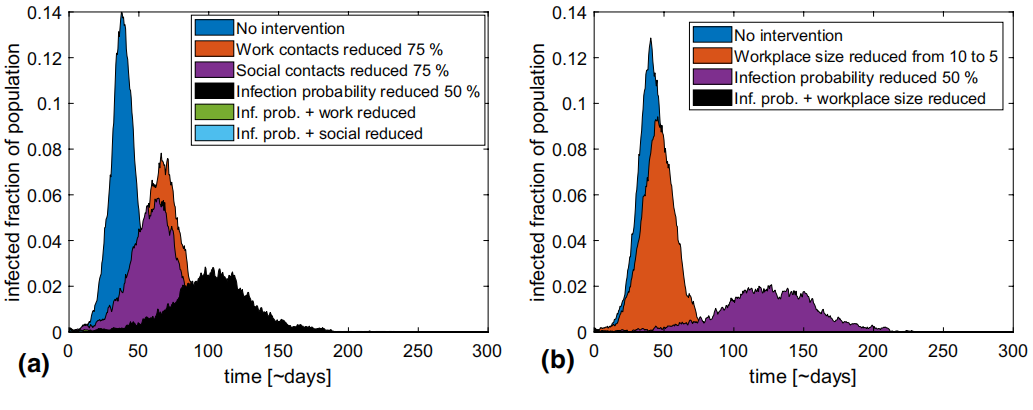
\includegraphics[scale = 0.5]{./img/paper/eilersen2020cost/1}
                    \label{fig:paper_result1}
                \end{figure}
                \begin{figure}[htbp]
                    \centering
                    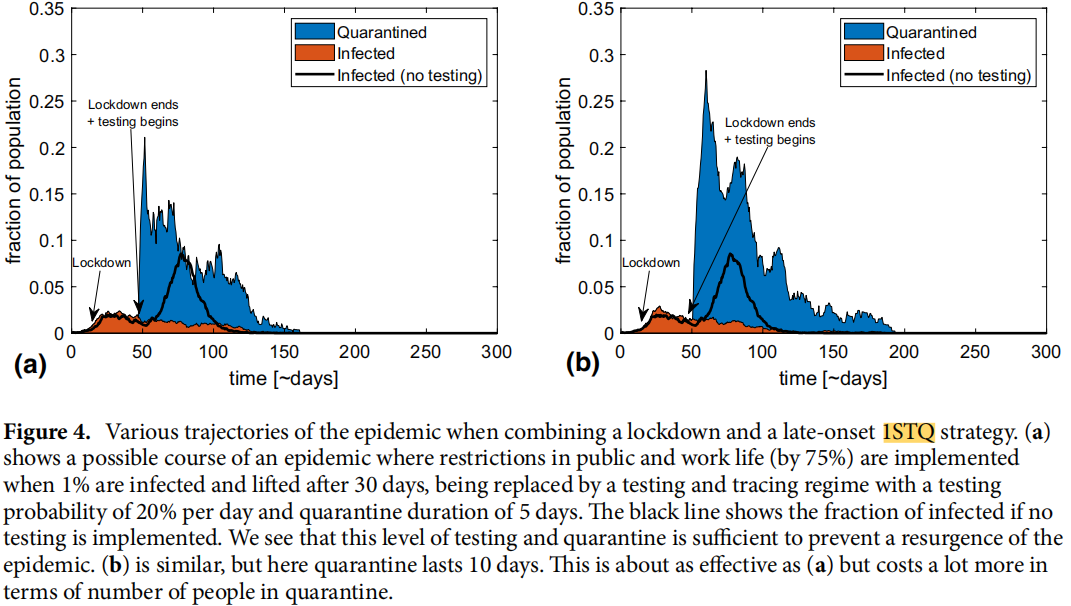
\includegraphics[scale = 0.3]{./img/paper/eilersen2020cost/2}
                    \label{fig:paper_result2}
                \end{figure}
                这种策略与overall Lockdown相比可以大大减少损失的工作日。如图\ref{fig:paper_result2}为采取封锁与未采取任何措施
                的结果,非常有意思的是,当Lockdown解除以后的30天开始检测隔离措施,隔离了大量的个体,最高甚至达到约
                30\%,而no testing 的感染人数尽管并没有隔离任由病毒在相同的环境下传播,但是最高的感染人数不过10\%,
                Quarantined 的节点是需要隔离5天的,无隔离措施的感染人数最高占约10\%,并持续时间大概在50天左右,而
                采取隔离措施的情况却是隔离人数最高甚至接近30\%,并持续约150天。我认为这样的隔离措施过于粗糙,假设
                病毒不会变异的情况下,尽管采取了这样的措施在50-100天的感染人数
                大大减少,隔离的人数和持续时间可以侧面反应成本,因此不难发现成本之大,也就是说尽管从结果上看采取1STQ的
                措施能大大减少损失的工作日,但是由于隔离的人数大大增加,损失了大量的劳动力。
        \section{针对前人的研究存在的问题提出的改进思路}
            \begin{figure}[htbp]
            \centering
            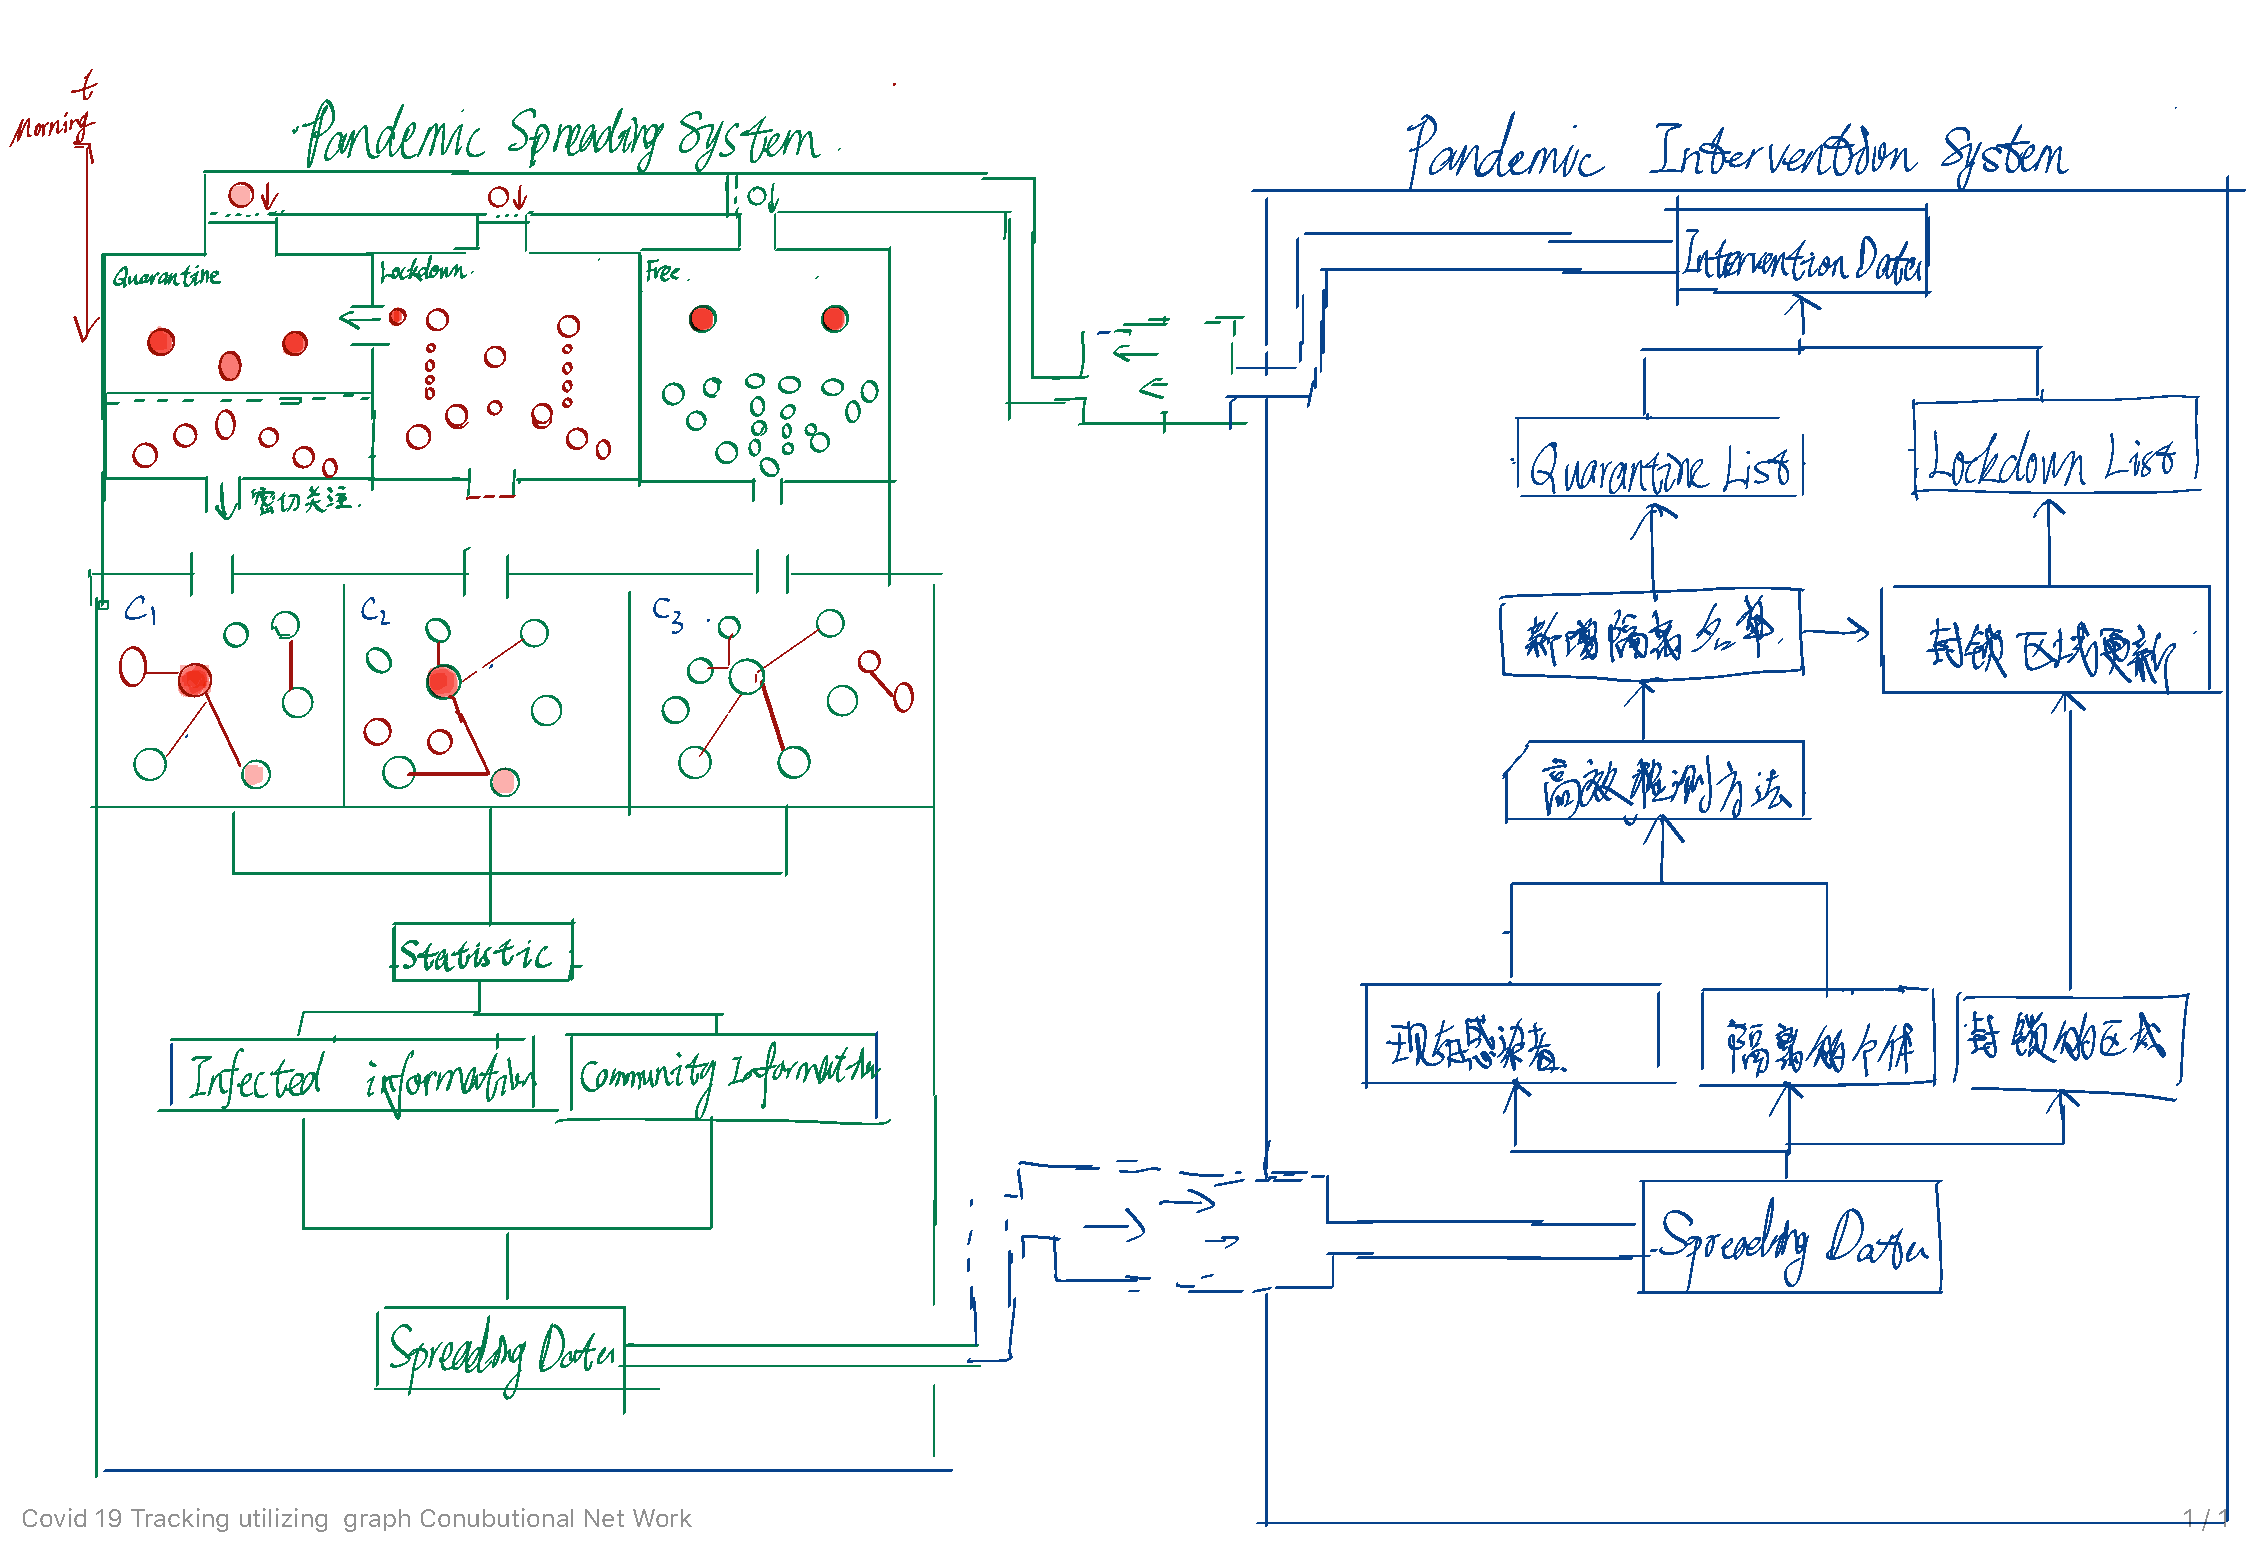
\includegraphics[scale = 0.40]{./img/workflow.pdf}
            \label{fig:workflow simulation}
            \caption{整个系统包括病毒传播系统(Pandemic Spreading System,PSS)和
            病毒干预措施系统(Pandemic Intervention System,PIS),在PSS中,红色的节点代表已确诊,红白的节点代表
            密切关注者,而绿白的节点代表易感人群和潜伏者。此外,流程图中设定了1个隔离区,1个封锁区,4个自由区作为示例。
            在隔离区,以虚实线分为必须隔离区和非必须隔离区,已确诊的节点隔离在必须隔离区,密切关注者则的行动与绿色的节点
            无差异,但必须采取戴口罩的措施,否则不能进入自由区。在自由区,节点可以根据偏好随意活动,
            只能跟同一区域内的节点接触。接着,每天统计感染者信息和所在的社区信息传输到PIS系统。收到了
            PSS传输的数据后,PIS根据现存的感染者和隔离的个体的状态信息,统计全部在自由区的有症状
            感染者所在的区域,对这些区域中所在的所有节点都进行检测并隔离,对于检测到为感染者的则安排到必须
            隔离区,而其他的节点则安排到非必须隔离区。接着,如果实行区域封锁,则将感染者所在区域进行全面封锁,
            除了已确诊的节点可以通往必须隔离区,封锁区域中的节点不能到其他的区域直到封锁期结束。}
        \end{figure}

%! Author = 207
%! Date = 2021/9/27

\part{数据介绍与动态网络构建}
    \chapter{数据介绍}
        \section{Gowalla Data}
        \section{Foursquare\_small Data}
        该数据集包括2012年4月12日至2013年2月16日从Foursquare收集的纽约市和东京的长期(约10个月)入住数据。
            其中文件名为dataset\_TSMC2014\_NYC.txt是纽约市的签入数据,一共227428行,
            文件名为dataset\_TSMC2014\_TKY.txt是东京的签入数据,一共573703行。
            地区偏移量的该地区(纽约市或东京),与UTC时间相差多少,单位为分钟,如-240,既该地区的当前时间等于UTC time的时间减去240分钟。

            % Please add the following required packages to your document preamble:
            % \usepackage{multirow}
            % \usepackage[table,xcdraw]{xcolor}
            % If you use beamer only pass "xcolor=table" option, i.e. \documentclass[xcolor=table]{beamer}
            \begin{table}[H]
            \begin{tabular}{llc}
            \hline
            数据字段                       & description   & 数据类型 \\ \hline
            User ID                    & 用户ID          & int  \\
            Venue ID                   & 场地ID          & str  \\
            Venue category ID          & 场地类别ID        & str  \\
            Venue category name        & 场地类别          & str  \\
            Latitude                   & 纬度            & int  \\
            Longitude                  & 经度            & int  \\
            Timezone offset in minutes & 时区偏移量(以分钟为单位) & int  \\
            UTC time                   & 世界标准时间        & str  \\ \hline
            \end{tabular}
            \end{table}

    \chapter{动态接触网络构建}
        \section{区域数据划分}
\subsection{判断该点是否在New York城市内}
在实际应用中,我们经常需要判断某个经纬度是否在某个区域内,而这个在程序中需要该区域的边界经纬度。
\subsubsection{获取区域边界}
我们可以从网站里获取经纬度:\url{https://nominatim.openstreetmap.org/ui/search.html}。在此网站内输入你想判断的区域名称,如,New York,点击Serach后再点击detail,复制该区域的OSM码。
\begin{figure}[H] %H为当前位置,!htb为忽略美学标准,htbp为浮动图形
\centering %图片居中
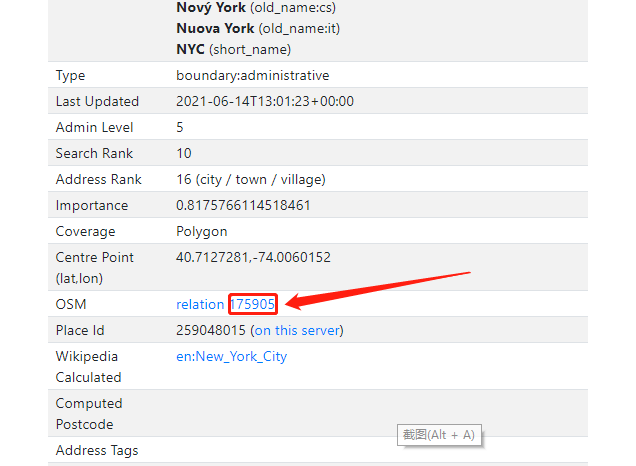
\includegraphics[width=0.4\textwidth]{./img/OSM ID.png} %插入图片,[]中设置图片大小,{}中是图片文件名
\caption{OSM 码} %最终文档中希望显示的图片标题
\label{Fig.OSM} %用于文内引用的标签
\end{figure}

在此网站输入OSM码\url{http://polygons.openstreetmap.fr/index.py},点击提交后就可以下载了。
\begin{figure}[H] %H为当前位置,!htb为忽略美学标准,htbp为浮动图形
\centering %图片居中
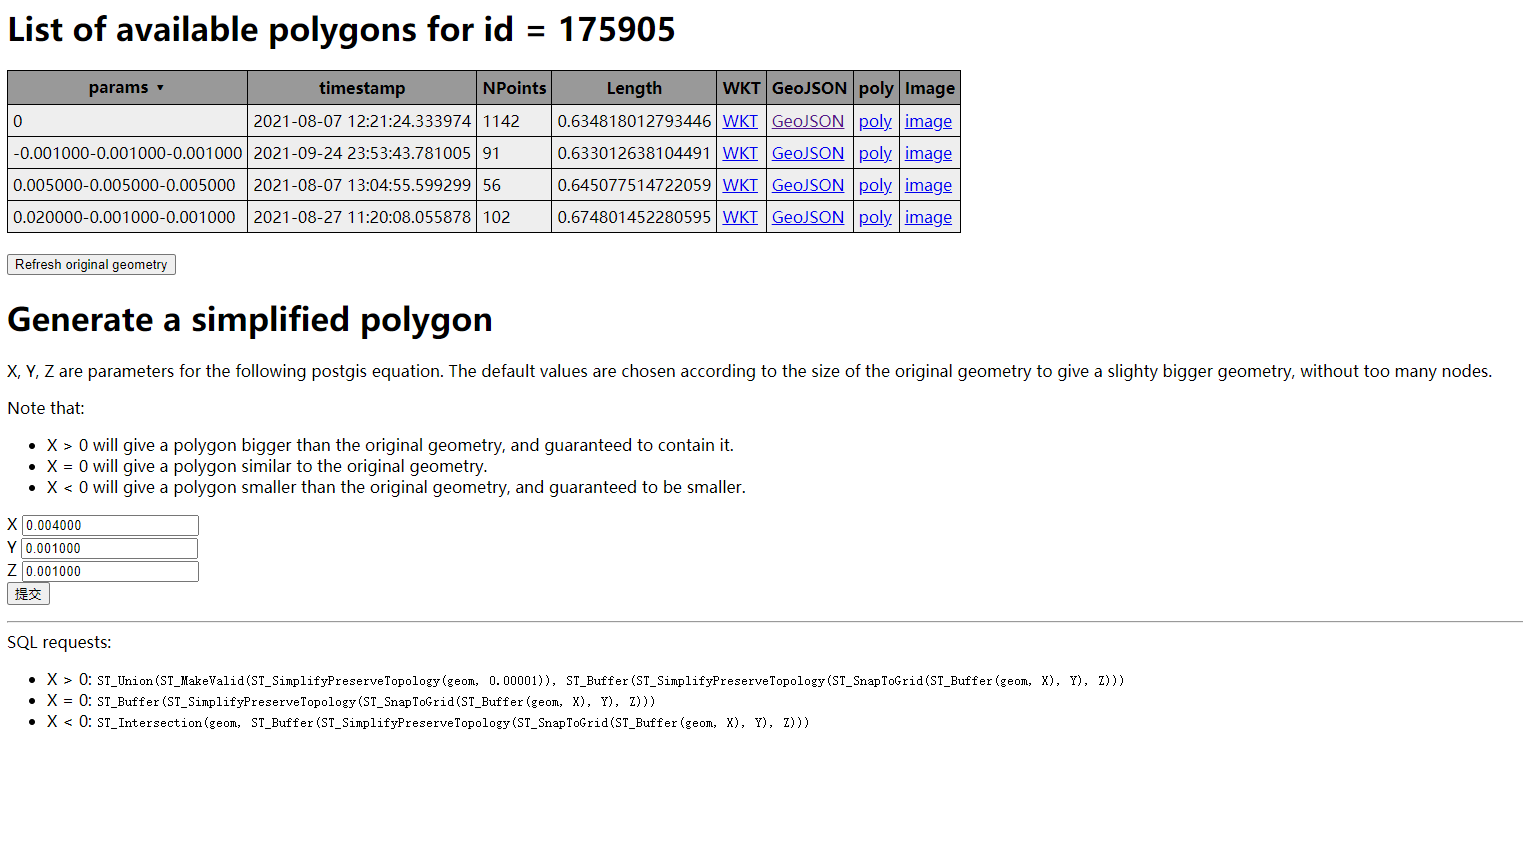
\includegraphics[width=0.4\textwidth]{./img/download.png} %插入图片,[]中设置图片大小,{}中是图片文件名
\caption{下载界面} %最终文档中希望显示的图片标题
\label{Fig.download} %用于文内引用的标签
\end{figure}

后续可以写一个方法,输入区域的名称后即可将该区域边界提取。

\subsubsection{判断方法}
由于New York城市是由多个点组成的一个不规则多边形,我们写了一个方法,用于判断某个经纬度坐标是否在New York这个城市里。此方法为射线法,步骤如下:
\begin{itemize}
\item[1)]从需要判断的点P向右引水平扫描线(即射线)。
\item[2)]计算此射线与多边形的交点个数c。
\item[3)]如果c为奇数,认为点P在多边形内;为偶数,则点P在多边形外。
\end{itemize}
如下图(a),c为奇数,所以P点在多边形外,图(b),c为偶数,所以P点在多边形内。


\begin{figure}[htbp]
\centering
\subfigure[P点在多边形外]{
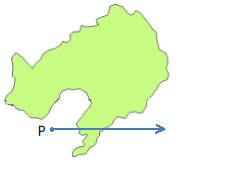
\includegraphics[width=0.3\textwidth]{./img/Ray_line_a.png}
%\caption{fig1}
}
\quad
\subfigure[P点在多边形内]{
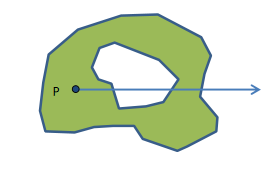
\includegraphics[width=0.3\textwidth]{./img/Ray_line_b.png}
}

\caption{射线法}
\end{figure}

在我们的数据集里,New York城市的边界是由很多个点(经纬度)组成的,我们可以把这些点连起来,就形成了一个多边形,再使用射线法去判断
。

我们的将此方法转化为程序的主要思路为:
\begin{itemize}
  \item [1)]
我们规定,点P为需要判断的点,$ x_p, y_p $分别为P的经度和纬度。$ N=\{P_n=(x_n,y_n)\mid n \in [0, k]\} $为New York城市的边界经纬度集合,其中k为New York城市经纬度的点的数量。

\item [2)]
按顺序将New York城市边界的每两个点连起来(如$ P_1, P_2 $或$ P_2, P_3 \cdots $),得到线段AB
\item [3)]
每次都用点P向右作射线,判断点P是否穿过线段AB
\item [4)]
如穿过,c加一,反之,c保持不变。
\item[5)]
直至后面将New York城市的所有点都判断后,再判断c的奇偶性,如c为奇数,则说明点P在多边形内,反之,点P在多边形外。
\end{itemize}
由于射线法本身存在缺陷,且在转化成代码时也会有相应的问题,我们在使用射线法前先进行了初步的判断以及排除一些情况:
\begin{itemize}
\item[1)]判断点P是否属于N,如是,则说明P在New York城市内。
\item[2)]判断点P是否属于线段AB上,如是,则说明P在New York城市内。(伪代码是否要给出来?)
\item[3)]点P正好位于线段AB的下端点,则在射线法里跳过此线段的判断。(怎么描述能更清楚?)
\item[4)]线段在射线的上方、线段在射线的下方、线段在射线的左方,则在射线法里跳过此线段的判断。


\end{itemize}
公式如下:

\[
isInRegion(N,P) = \begin{cases} in, & 2\nparallel \sum\limits_{n=1}^{k} M(P_n, P_{n+1},P)
 \\
out, & 2\parallel \sum\limits_{n=1}^{k} M(P_n, P_{n+1},P)
\end{cases}
\]
其中,k为New York城市经纬度的点的数量, $ M(P_n, P_{n+1},P) $的作用为计算每一条线段与P是否有交点,公式在此给出:
\[
M(P_n, P_{n+1},P) = \begin{cases}
0, & x_{meet}< x_p
 \\
1, & x_{meet}> x_p
\end{cases}
\]
\[
x_{meet} = x_n -\frac{x_n - x_{n+1}}{y_n - y_{n+1}}(y_n - y_p)
\]
其中,$ x_{meet} $为P点的射线与线段AB的交点的横坐标,其原理为三角形的相似性,原公式如下:
\[
\frac{x_n - x_{n+1}}{y_n - y_{n+1}}= \frac{x_n - x_{meet}}{y_n - y_p}
\]

\begin{figure}[H] %H为当前位置,!htb为忽略美学标准,htbp为浮动图形
\centering %图片居中
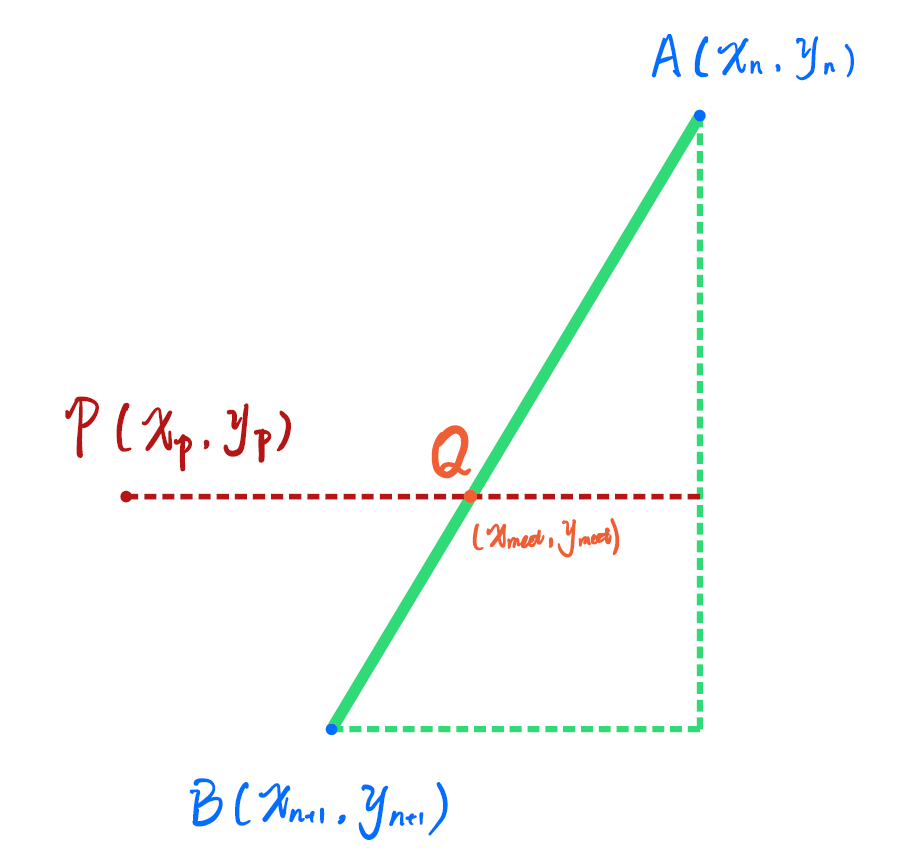
\includegraphics[width=0.4\textwidth]{./img/similar_triangles.png} %插入图片,[]中设置图片大小,{}中是图片文件名
\caption{similar triangles} %最终文档中希望显示的图片标题
\label{Fig.main2} %用于文内引用的标签
\end{figure}



在上面的公式里,$ isInRegion(N,P) $中,如果 $ \sum\limits_{n=1}^{k} M(P_n, P_{n+1},P) $能被2整除,说明c为偶数,所以我们通过射线法可以知道点P在该区域内,反之,则在该区域外。


%此外,由于射线法是有一定的缺陷的,当该点在多边形上时,并不能准确判定该点是否在多边形内,因此,我们在使用射线法前先进行简单判断,如果点P在多边形上,则认为该点是在该区域内,反之,则使用射线法进行进一步的判断。判断公式如下
%
%\IncMargin{1em}
%\begin{algorithm}[H]
%%\SetAlgorithmName{\color{red} \textbf{算法}}{}{}
%
%\SetKwData{Left}{left}\SetKwData{This}{this}
%\LinesNumbered
%\SetKwData{Up}{up}
%\SetKwFunction{Union}{Union}\SetKwFunction{FindCompress}{FindCompress}
%\SetKwInOut{Input}{Input}
%\SetKwInOut{Output}{output}
%\Input{Longitudes $ X $; \newline Latitudes $ Y $; \newline P \quad $ x_p, y_p $}
%\
%%\Output{A partition of the bitmap}
%%\BlankLine %间距
%%\emph{special treatment of the first line}\;
%\For{$ n=1,2,\ldots ,N $}{
%\uIf{$ x_p >= min(x_n, x_{n+1}) \quad  and \quad x_p <= max(x_n, x_{n+1})$}
%{\label{lt}
%\uIf{$ y_p >= min(y_n, y_{n+1}) \quad  and \quad y_p <= max(y_n, y_{n+1})$}
%{\label{lt}
%\uIf{$ (x_p - x_n)(y_{n+1}-y_n) - (x_{n+1}-x_n)(y_p - y_n) = 0 $}{\KwRet{$ True $}}
%}
%}}
%
%\caption{isInlinesegment Function}\label{isInlinesegment Function}
%\end{algorithm}\DecMargin{1em}
%
%
%公式解释,在判断一个点是否在一条线段上,有两个条件
%\begin{itemize}
%  \item [1)]
%  该点在以此线段为对角线的矩阵内(第一、第二个if判断条件)
%  \item [2)]
%  该点与此线段的其中一端相连形成的线段B,把此线段B与原线段求叉积,若叉积为0时(第三个if判断条件)
%\end{itemize}

    

%! Author = 207
%! Date = 2021/9/27

\part{基于动态网络的传播模型}


    

%! Author = 207
%! Date = 2021/9/27

\part{干预措施}
    \chapter{邻接检测}
    \chapter{区域检测}
        \section{数据分析}
            \subsection{个体不带口罩,政府执行区域检测隔离措施}
                在个体不带口罩,政府执行区域检测隔离措施的情况下,我们对各个状态(SEAIR)进行分析,画出了下列图片,其中,Y轴为某状态当前人数/总人数,
                X轴为iteration,即迭代的次数。
                \begin{figure}[H]
                    \centering
                    \subfigure[S]{
                    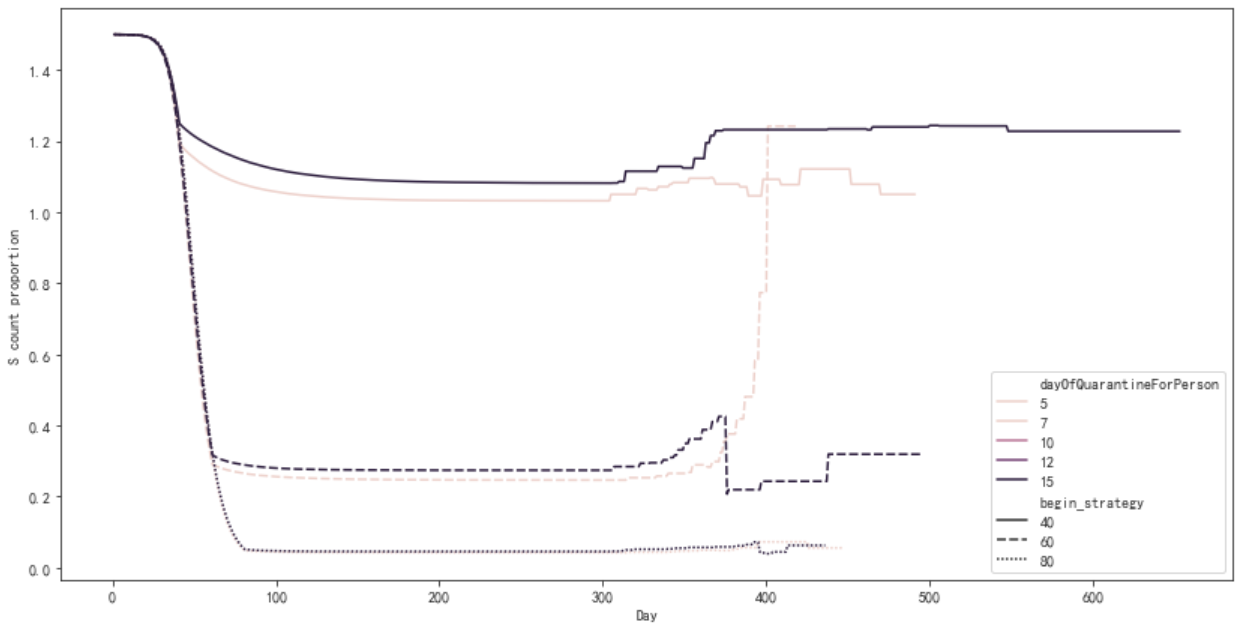
\includegraphics[width=5.5cm]{img/S}
                    %\caption{fig1}
                    }
                    \quad
                    \subfigure[E]{
                    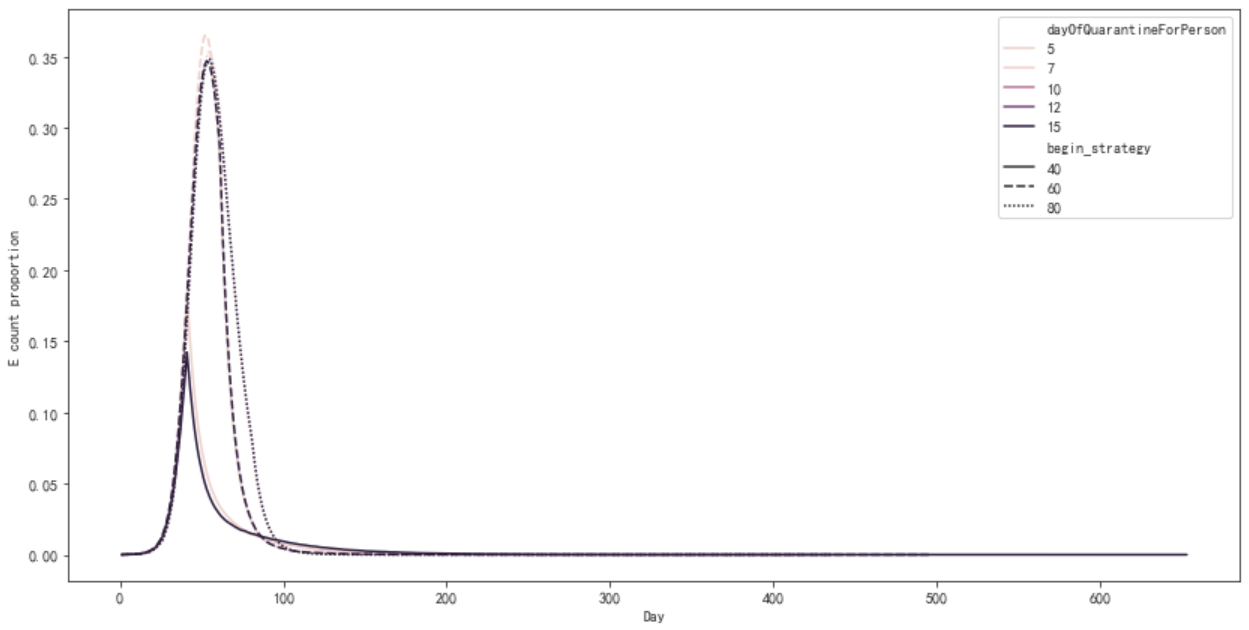
\includegraphics[width=5.5cm]{img/E.png}
                    }
                    \quad
                    \subfigure[A]{
                    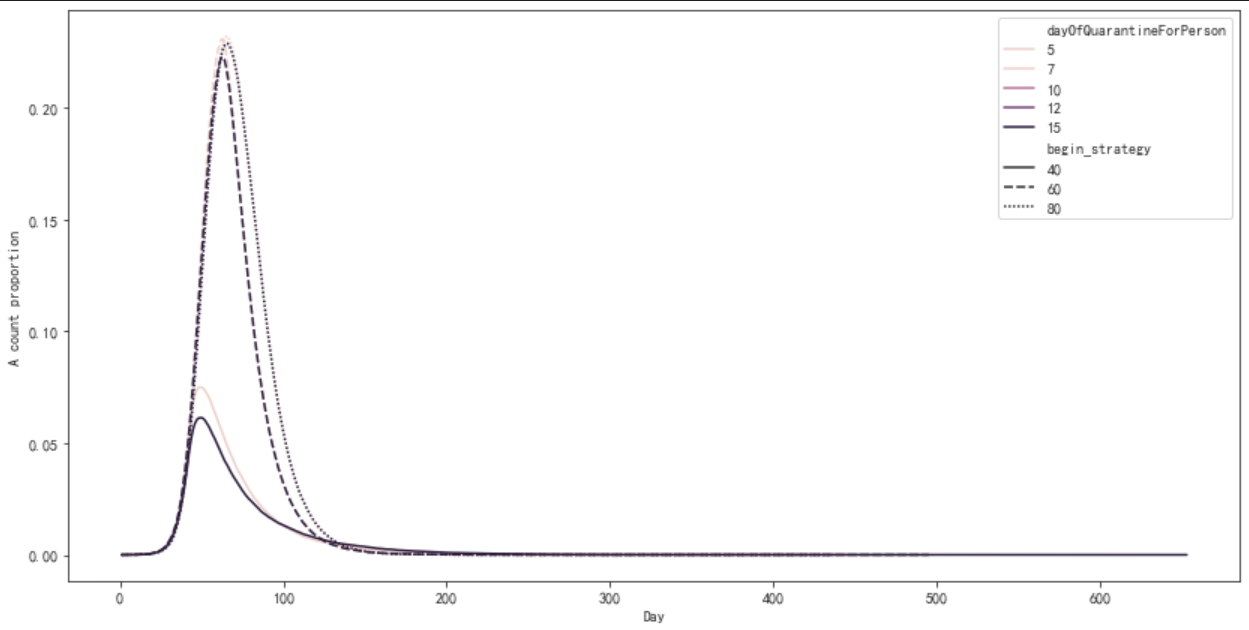
\includegraphics[width=5.5cm]{img/A.png}
                    }
                    \quad
                    \subfigure[I]{
                    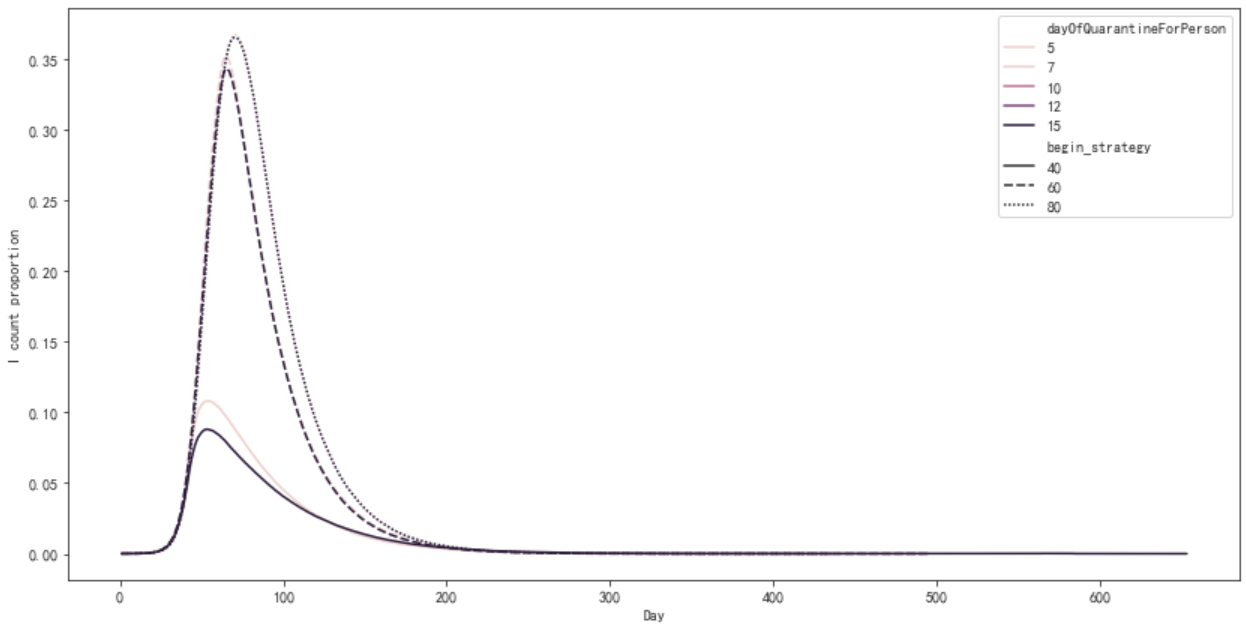
\includegraphics[width=5.5cm]{img/I.png}
                    }
                    \quad
                    \subfigure[R]{
                    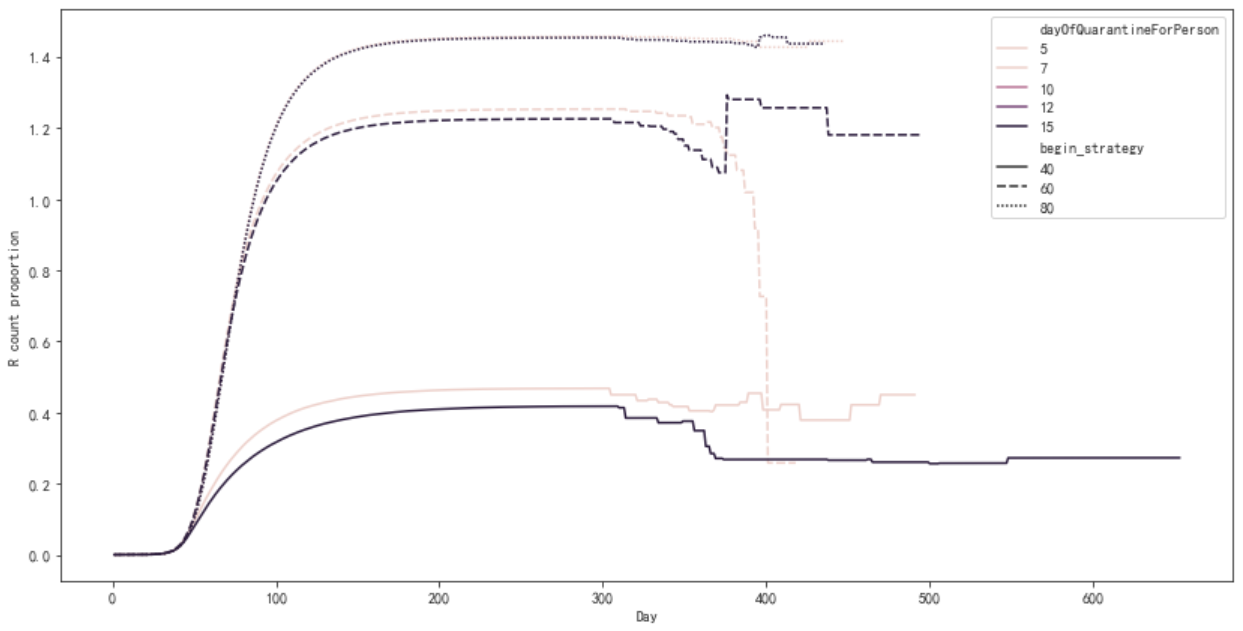
\includegraphics[width=5.5cm]{img/R}
                    }
                    \caption{各个状态人数占总人数}
                \end{figure}

                从图中可以看出,处于S状态和R状态图可以明显看到在iteration>300时,曲线的变化不像以往缓慢,S占比开始上升,而R开始下降,而在iteration>400时,
                S和R都开始出现垂直上升或下降或者暂缓不变的现象。于是,我们将S和R的占比画在同一幅图里,以观察他们的之间的关系。
                \begin{figure}[H]
                    \centering
                    \subfigure[7]{
                    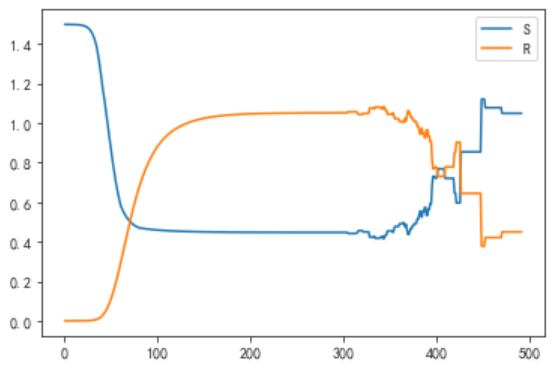
\includegraphics[width=5.5cm]{img/7}
                    %\caption{fig1}
                    }
                    \quad
                    \subfigure[14]{
                    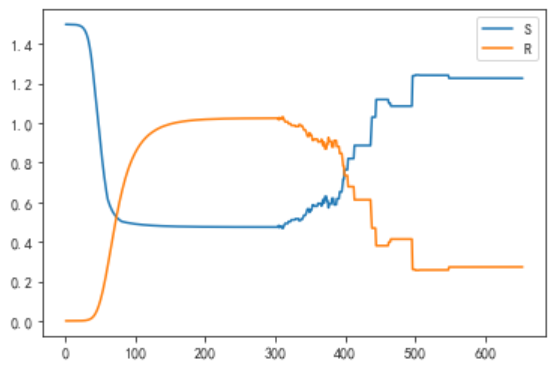
\includegraphics[width=5.5cm]{img/14}
                    }
                    \caption{处于S状态和R状态占比分析图}
                \end{figure}
                可以看到,S状态与R状态在dayOfQuarantineForPerson=7或dayOfQuarantineForPerson=14时都表现出对称性,目前未发现出现此现象的原因。
    \chapter{基于历史轨迹的区域检测}
    \chapter{基于图神经网络的区域检测推荐}


    

%! Author = 207
%! Date = 2021/9/27

\part{实验结果}
    \chapter{模型参数设置}
    \chapter{结果分析}


    

%! Author = 207
%! Date = 2021/9/27

\part{Discussion and Conclusion}



    

%----------------------------------------------------------------------------------------
%	INDEX
%----------------------------------------------------------------------------------------


\cleardoublepage % Make sure the index starts on an odd (right side) page
\phantomsection
\setlength{\columnsep}{0.75cm} % Space between the 2 columns of the index
\addcontentsline{toc}{chapter}{\textcolor{ocre}{Index}} % Add an Index heading to the table of contents
\printindex % Output the index
%----------------------------------------------------------------------------------------

\end{document}
